\chapter{Surface current and power loss in a conductor}
In our previous chapter we talked about Power Flow in an electromagnetic wave and poynting vector for electromagnetic waves. The poynting vector tells the density of power flow and its direction tells us the direction of the power at any location in space.\\

In this chapter we will talk about surface current and power loss in a conductor.\\

We have always wondered how much power is lost in a conducting surface when an electromagnetic wave is incident on the conducting surface, the origin of surface current, do we really have surface current in practice and many more.\\

Surface Current is essentially a phenomenon which lies on the surface of the medium. This is a phenomenon which is for ideal conducting surface.\\

We will begin this chapter from the volume current density inside a conductor, we know the concept of skin depth in a good conductor, from there we will find out the current which is the surface current and say in practical systems the concept of surface current is very useful in finding out how much losses takes place in a conducting surface. First we will discuss surface current and then go to power loss in a conducting surface.\\

We established that $\hat{n}$x$\hat{H}$ gives the direction of the surface current. $\hat{n}$x$\hat{H}$ gives us the direction which goes into the paper as shown in the image below\\
\begin{figure}
\centering
\textsc{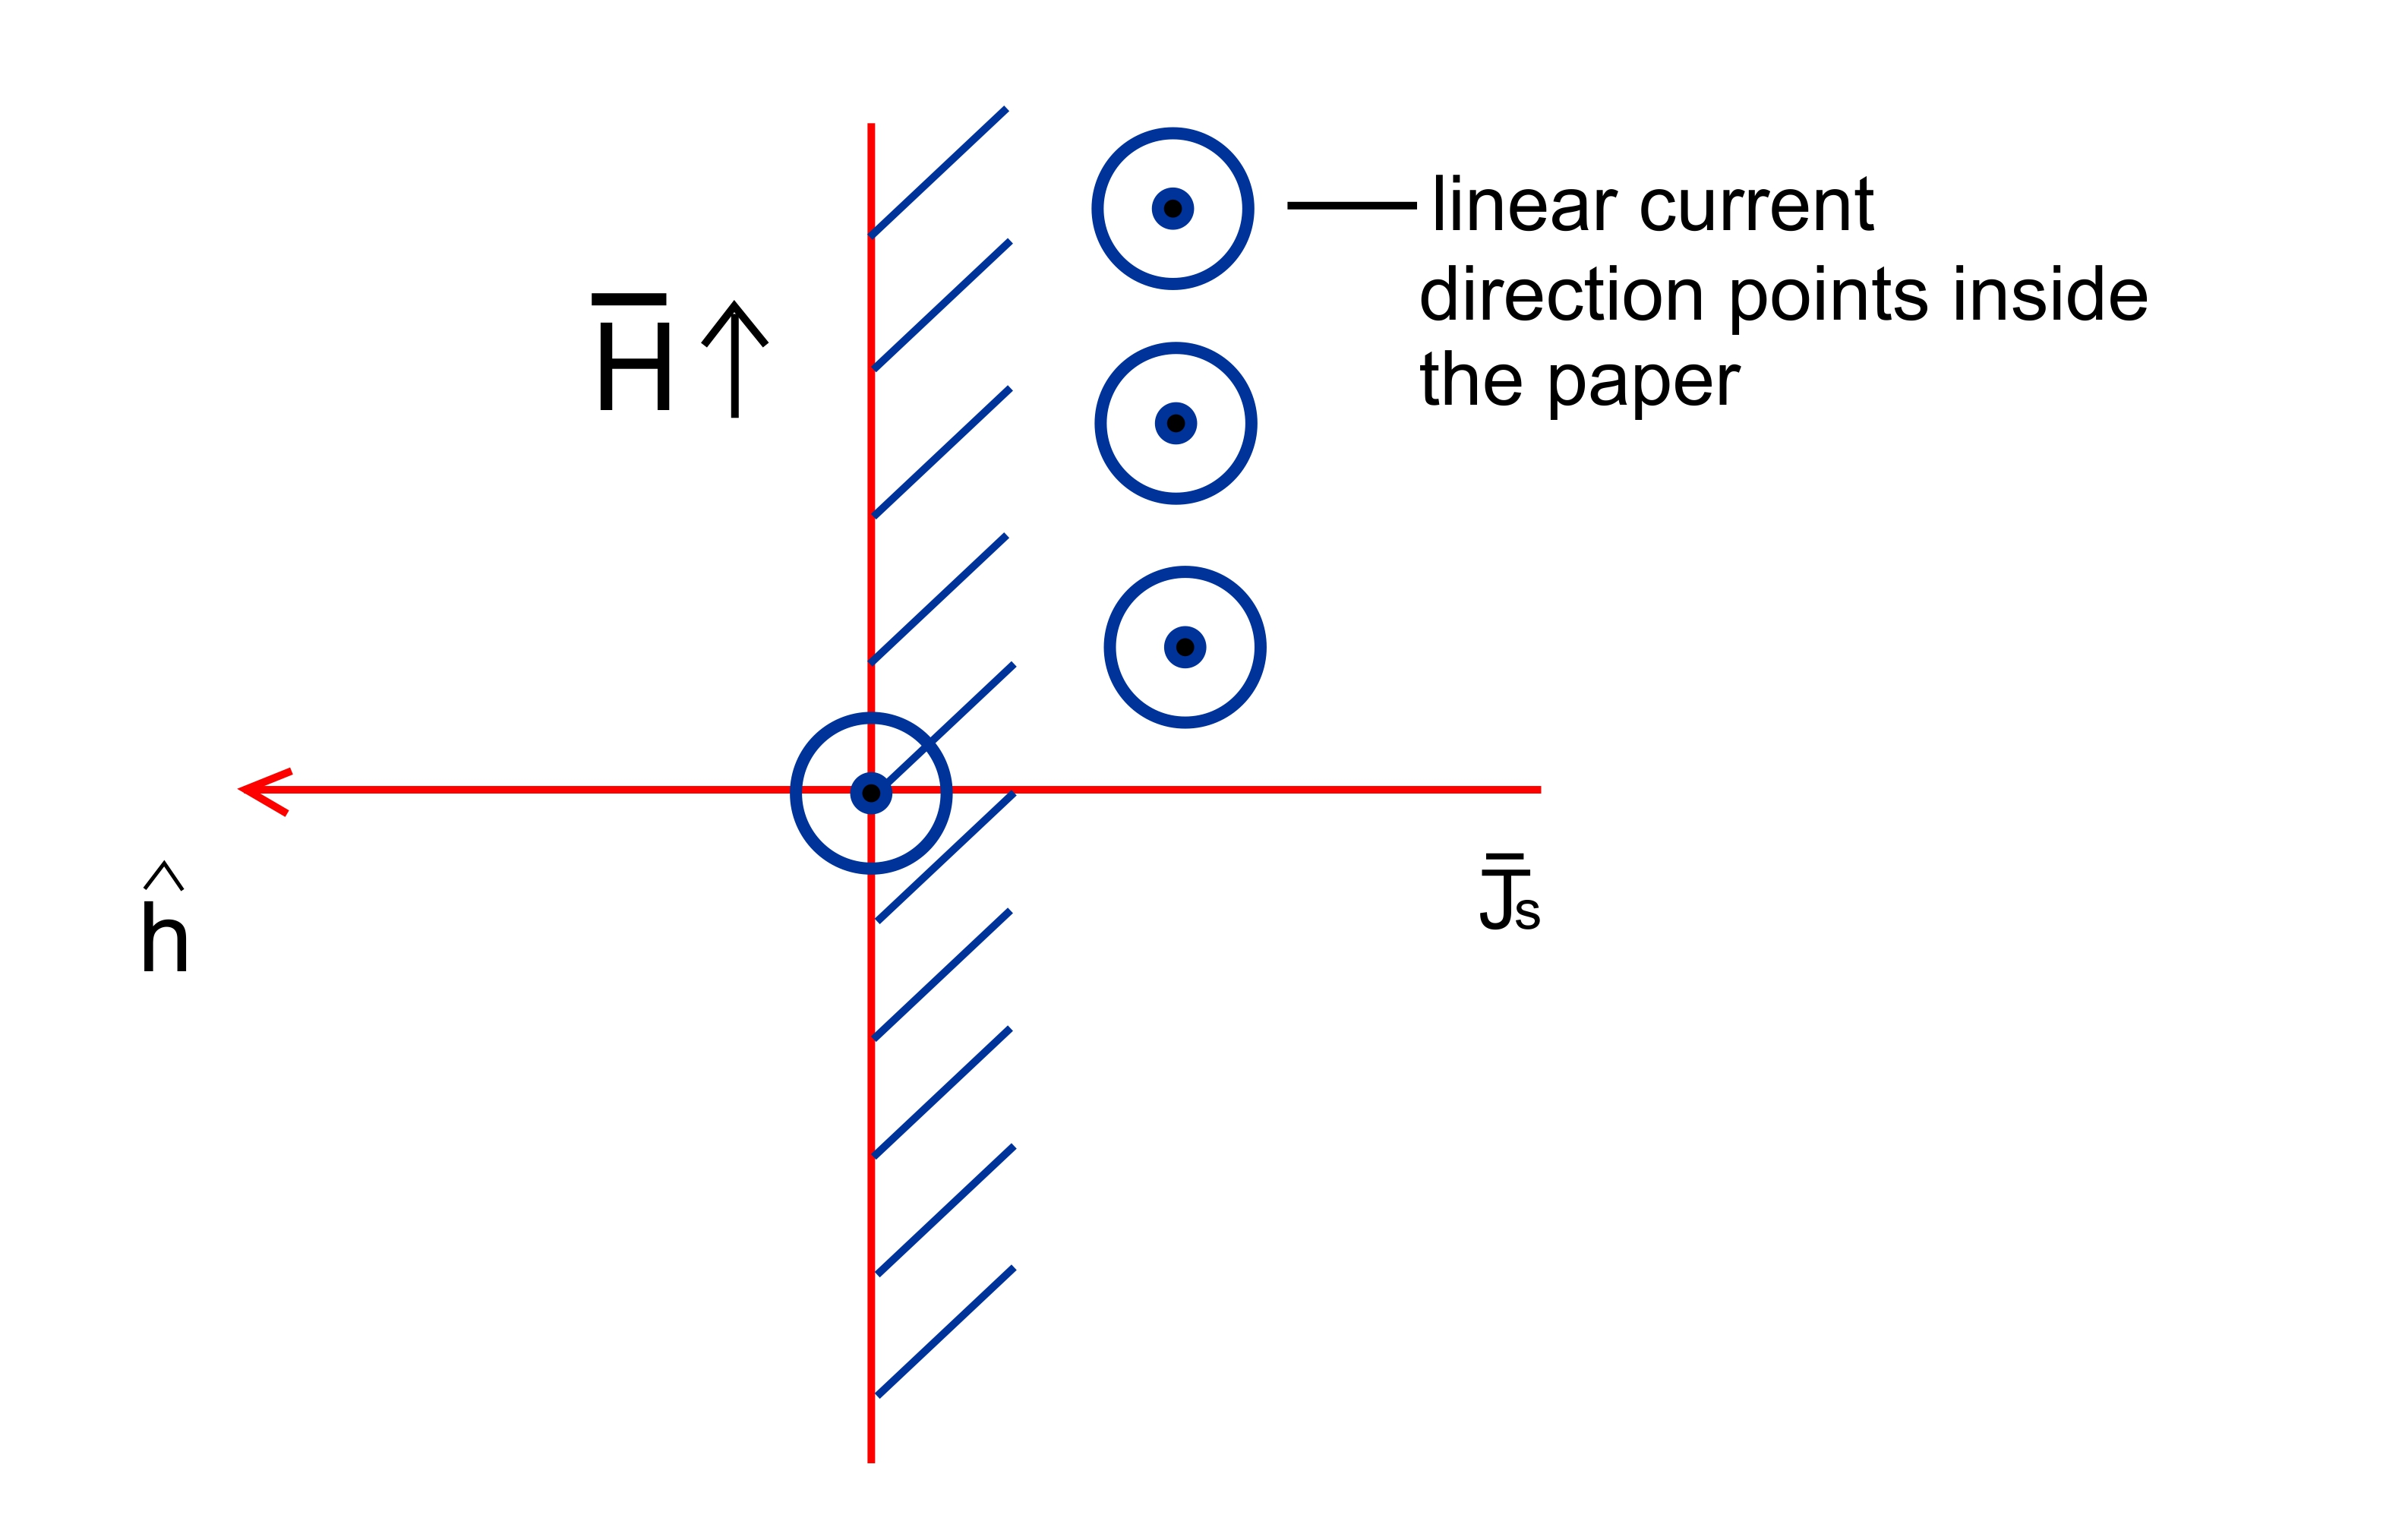
\includegraphics[scale=0.5]{Bello281}}
\caption{Direction of the surface area }
\end{figure}\\

This gives the linear surface density $\bar{J}$s we talked about when we dealt with boundary condition. If the surface current is flowing here, what is the driving mechanism for this surface current?\\

It is already established that this surface current phenomenon is associated with infinite conductivity. So if we take an ideal conductor, then maybe at some point of time, instantaneously, there are some electric field that existed in the medium and since it was a very short lived phenomenon we had electric and magnetic field together.\\
 For the momentary existence of electric field, it would put the charges into motion, which would constitute this current and since the conductivity is infinite, even if the electric field doesn't exist anymore when the charges are put in motion, the charges will keep moving for infinite time. That means they would have current. So when the conductivity is infinite, one may visualize this that at some extent of time, some electric field induced motion to these charges. The charges were set in motion and they kept moving which is essentially the surface current and this is balanced by the magnetic field and $\hat{n}$x$\hat{H}$ essentially gave us that current density $\bar{J}$.\\
 
  There are two situations now that we have tangential component of electric field on the conducting surface which is zero but there are no surface currents and the tangential component of electric field is zero and there is surface current. So both situations, we have the tangential component of electric field to be zero for ideal conductors. In one case, we have surface current and in the other case, we do not have surface current. If we have surface current, then it must be balanced by the magnetic field. So if we have a magnetic field tangential to the conducting boundary, then we will have surface current otherwise we will not have surface current. Now this is a hypothetical situation of when surface current is truly flowing on the surface. We see what happens if we take a good conductor, can we still make use of this concept called surface current? It is very clear that if we have a conductivity which is not infinite, then because of electric field there will always be a finite conduction current density inside the material of the conductor. Also the skin depth is of finite width, that is this phenomenon is not a true surface phenomenon (this requires zero thickness for skin depth). From the diagram of the conductor shown below. Let \textbf{Z} \textgreater 0 represent the conductor.\\
\begin{figure}
\centering
\textsc{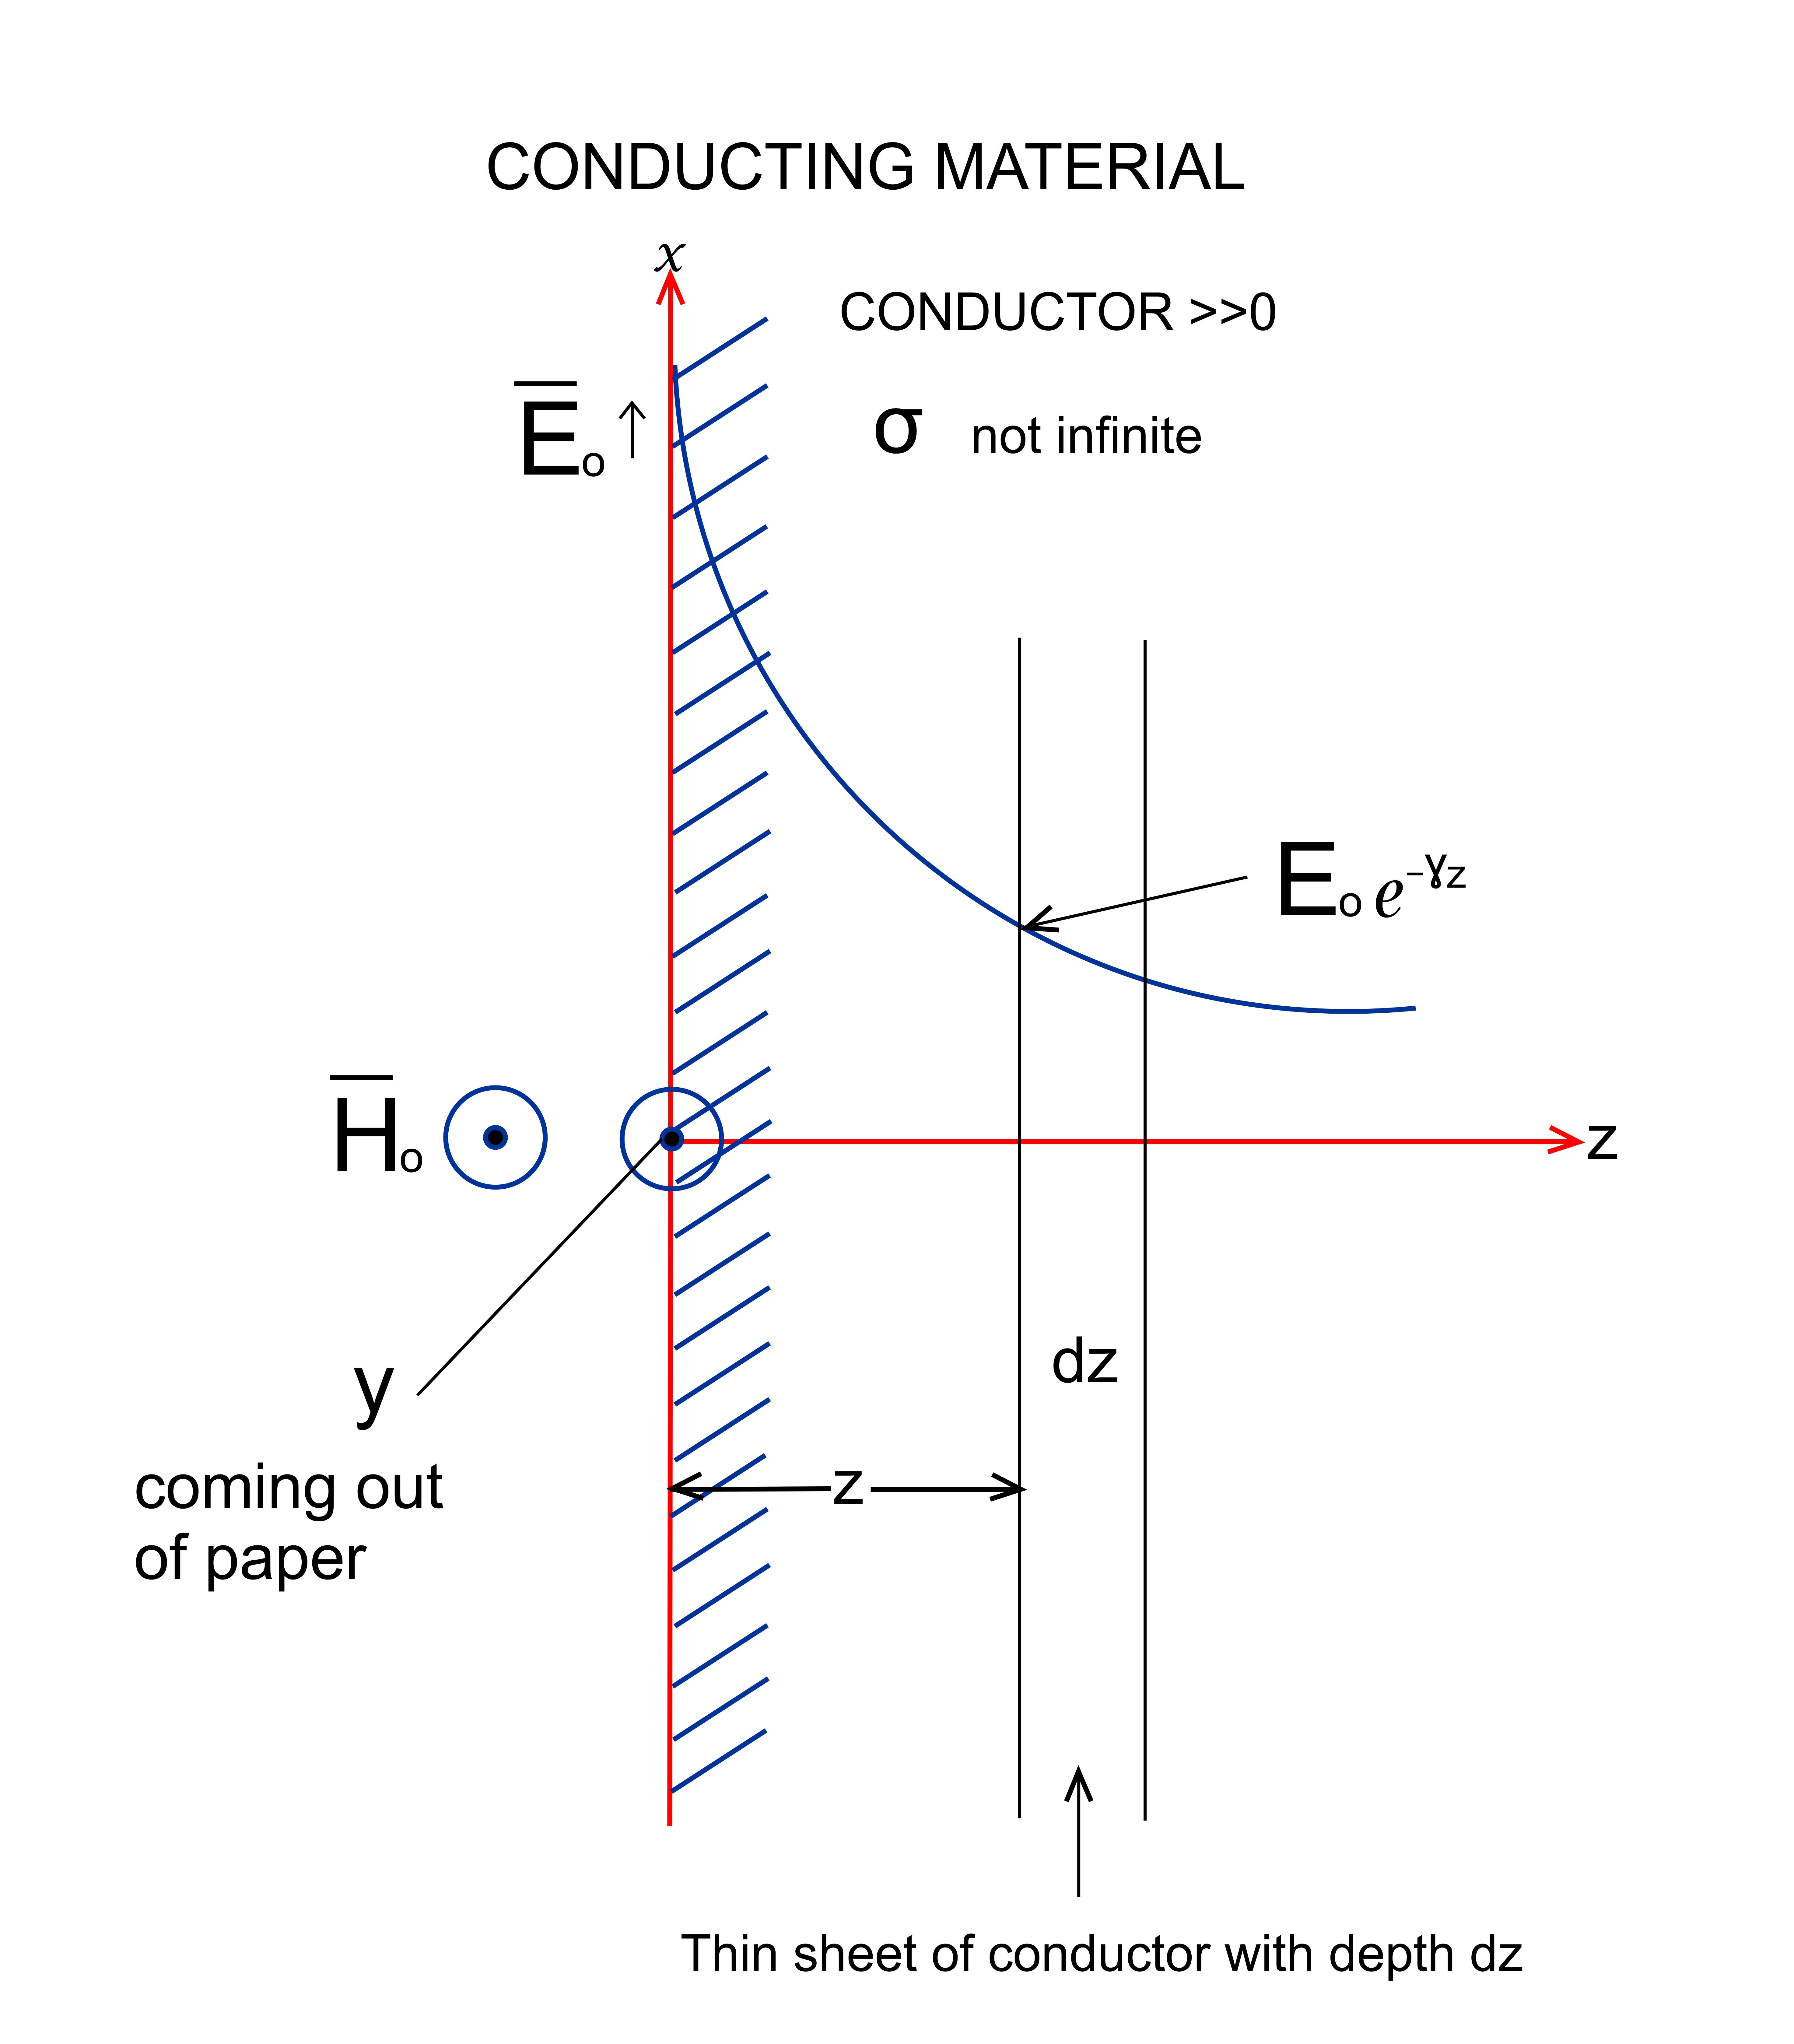
\includegraphics[scale=0.1]{Bello282}}
\caption{A conductor shown in three dimension}
\end{figure}	
If we have electric field in this conductor for a finite $\sigma$ not $\infty$. Then the tangential component of \textbf{E} on this surface is not zero (very very small but not zero as for ideal conductor with $\infty$ conductivity). Let \textbf{E} be in \textbf{x} direction and \textbf{H} in \textbf{y} direction. The \textbf{E} field dies down exponentially as we go into the conductor as shown above. \textbf{E} dies down at $\bar{E}_0^{-\partial z}$. Once we know the electric field value at the surface of the conductor, we have

\begin{align}
\gamma=\sqrt{\textit{j}\omega\mu\sigma}
\end{align}
for a good conductor, $\sigma$ is very large. $\gamma$=$\alpha$+$\beta$ to get
\begin{align}
\gamma=\sqrt{\frac{\omega\mu\sigma}{2}}+\textit{j}\sqrt{\frac{\omega\mu\sigma}{2}}=\alpha+\textit{j}\beta
\end{align}\\

Since the current flow in the direction of the electric field $\hat{x}$, we have a conduction current density $\bar{J}$=$\sigma\bar{E}_o$ which varies exponentially as we go deeper inside the conductor. We can take a thin sheet with depth of \textbf{dz}. The conduction current $\bar{J}$=$\sigma\bar{E}_o$\textit{e}$^{-\gamma z}$. So if we ask what is the current flowing in the sheet in the xy plane per unit area. From which we can find out the total current flowing in the whole z below a unit area of the xy plane and the current flows in x direction. So if we take the conduction current density and integrate over the depth, we get the total current flowing on the surface xy. If we take that surface as a unit surface, then the current that is flowing is with respect to that unit area. So we can work for dz region the conduction current density\\\\ $\bar{J}$(z) = $\sigma$$\bar{E}$ = $\sigma\bar{E}_o$\textit{e}$^{-\gamma z} \hat{x}$ = $\sigma\bar{E}_o$\textit{e}$^{-\gamma z}$\textit{e}$^{-j\beta z}$.\\\\
 Unit depth in y direction and width dz represent the area that $\hat{J}$ flows through. For this Area=1x\textbf{dz}=\textbf{dz}. Since current flows in $\hat{x}$ direction, the area normal to this flow is in yz plane and we take a unit y depth in  axis. So that current in slab of unit depth in y direction along the whole z plane is integration over entire z.\\

\begin{align}
\textbf{I}(z)=\bar{J}(z)\times Area (Area=1\times dz)\\
\textbf{I}(z)=\bar{J}(z)dz\\
\textbf{I}(z)=\sigma\bar{E}_0\textit{e}^{-\gamma z} \hat{x}
\end{align}
The above equation is the per unit length in y direction, the total current flowing in the surface is the surface current. Note there is no true surface current, current flow into the depth of z but dies down very fast. Hence the little current flow is limited to small dz on the surface of the conductor with large conductivity, we know that the skin depth is very small, so the current flow is confined to the surface, but not truely confined to the surface, but to a skin depth from the surface.\\
Surface current,
\begin{align}
\bar{J}s=\int\limits_o^\infty\sigma\bar{E}_o\textit{e}^{-\gamma z}dz\\'{s}\u{o} \hat{x}=\frac{\sigma\bar{E}_o}{-\gamma}[\textit{e}^{-\gamma z}]_0^\infty \hat{x}\\
\bar{J}=\frac{\sigma}{\gamma}\bar{E}_0\hat{x}
\end{align}


Though we call $\bar{J}$s surface current density, it is clear that it is not truly a surface phenomenon. It has all the property related to magnetic field, which is tangential component of the magnetic field to the surface. So it should satisfy the relationship of $\hat{n}$x$\hat{H}$=$\bar{J}$s. So if 
$\bar{J}$=$\dfrac{\sigma}{\gamma}$
$\bar{E}$$_o$$\hat{x}$ must serve as surface current density, it must be related to the magnetic field and satisfy $\hat{n}$x$\hat{H}$=$\bar{J}$s.\\

Since we have electric field which is $\bar{E}$$_o$ on the surface and magnetic field $\bar{H}$$_o$, with wave traveling in the Z direction for transverse electromagnetic wave and the medium unbound, $\dfrac{\bar{E}_o}{\bar{H}_o}$ must satisfy the relationship of being of equal to the intrinsic impedance of the media.\\
For a good conductor, intrinsic impedance
\begin{align}
\eta_{c}=\sqrt{\dfrac{j\omega\mu}{\sigma}}\\
H_{o}=\dfrac{E_{o}}{\eta_{c}}
\end{align} 
but $\gamma$=$\sqrt{j\omega\mu\sigma}$\ so,\\
\begin{align}
\eta_{c}=\sqrt{\dfrac{j\omega\mu}{\sigma}}\equiv\sqrt{\dfrac{j\omega\mu\sigma}{\sigma^{2}}}=\dfrac{\gamma}{\sigma}\\
\eta_{c}=\dfrac{\gamma}{\sigma}
\end{align}
From,
\begin{align}
H_{o}=\dfrac{E_{o}}{\eta_{c}}=\dfrac{\sigma E_{o}}{\gamma}\\
\end{align}
compared to 
\begin{align}
\bar{J}s=\dfrac{\sigma}{\gamma}E_{o}\hat{x}\\
\lvert H_{o}\rvert=\dfrac{\sigma}{\gamma}\lvert E_{o}\rvert=\rvert \bar{J}s\rvert.
\end{align}\\

So one relationship we wanted was that if $\bar{J}$s is surface current density the way we have visualized it. Then it must be related to the magnetic field and we have just shown that $\lvert$ H$_{o}$$\rvert$=$\rvert$$\bar{J}$s$\rvert$. The second requirement is that $\hat{n}$x$\hat{H}$=$\bar{J}$s i.e $\hat{n}$x$\hat{H}$  must give surface current direction $\hat{J}s$ was in direction of \textbf{E} that is $\hat{x}$, so surface current density $\hat{J}$s had $\hat{x}$ direction also. \textbf{H} is $\hat{y}$ oriented here. The unit normal to the conducting surface is $\hat{n}$=-$\hat{z}$. say $\hat{n}$x$\hat{H}$=-$\hat{z}$ x $H_{o}$$\hat{y}$, the $\hat{x}$ gives direction of $\bar{J}$s. That means that $\bar{J}$s=$\dfrac{\sigma}{\gamma}$$E_{o}$$\hat{x}$ has all the characteristics of a surface current density. So $\hat{n}$x$\bar{H}$ gives the surface current. The magnitude of the magnetic field should be equal to that of the surface current density. This is the reason that though $\bar{J}$s=$\dfrac{\sigma}{\gamma}$$E_{o}$$\hat{x}$ is not a true surface current, we use it as a surface current. Also when conductivity is very large, this current is effectively confined to a very thin layer called skin depth. As we have seen earlier, if we go to frequency like 300Mh$_{z}$, skin depth lies in few micron range. So essentially this is a current flowing through a very thin sheet on the surface of the conductor. Also, it has the characteristics of a true surface current that is, it is related to the magnetic field and $\hat{n}$ x $\bar{H}$ gives its direction. So this quantity can be used as the surface current in a good conductor. In true sense of it, there is no surface current for a good conductor. We do not have true surface current because conductivity is always finite, we make use of the quantity $\bar{J}$s as surface current and we can do the calculation by using the concept of surface current.\\

Once we get surface current, we define a quantity called \textbf{SURFACE IMPEDANCE} which is a boundary parameter for this boundary. This is useful whenever we do the power calculation on conducting surface.\\
Surface impedance
\begin{align}
Z_{s}=\dfrac{E_{tangetial}}{\bar{J}s}
\end{align}
\begin{align}
\bar{J}s=\dfrac{\sigma}{\gamma}E_{o}\hat{x}
\end{align}
has $\dfrac{A}{m}$ as its unit. So dimension of surface current density is a linear density.
\begin{align}
Z_{s}=\dfrac{V/m}{A/m}=\dfrac{V}{A}=\Omega ohms
\end{align}
So the quantity Z$_{s}$ is some impedance. If we know the tangential component of electric field, then the surface current can be obtained from what is called the surface impedance or vice versa.\\
\begin{align}
Z_{s}=\dfrac{E_{o}}{\dfrac{\sigma}{\gamma} E_{o}}=\dfrac{\gamma}{\sigma}=\dfrac{\sqrt{j\omega\mu\sigma}}{\sigma}=\sqrt{\dfrac{j\omega\mu}{\sigma}}=\eta_{c}
\end{align}
So for a good conductor, the intrinsic impedance of the medium is same as surface impedance. Later we set that surface impedance concept is used to calculate the power loss. If we know tangential component of electric field and know the conductivity, we can calculate the intrinsic impedance of the medium which is same as surface impedance.\\
Once we have the surface current density $\bar{J}$s, then we ask how much is the power loss because of this surface current density flowing on this conductor. We take a surface of unit area, how much is the power loss in this unit area of the conducting surface? Since the current is flowing into the depth of the conductor, the power loss is not only taking place on the surface, it takes place all along the depth of the conductor. We ask what is the total loss if we take the total depth of the conductor? We take a unit area shown of thickness dz shown below.

\begin{figure}
\centering
\textsc{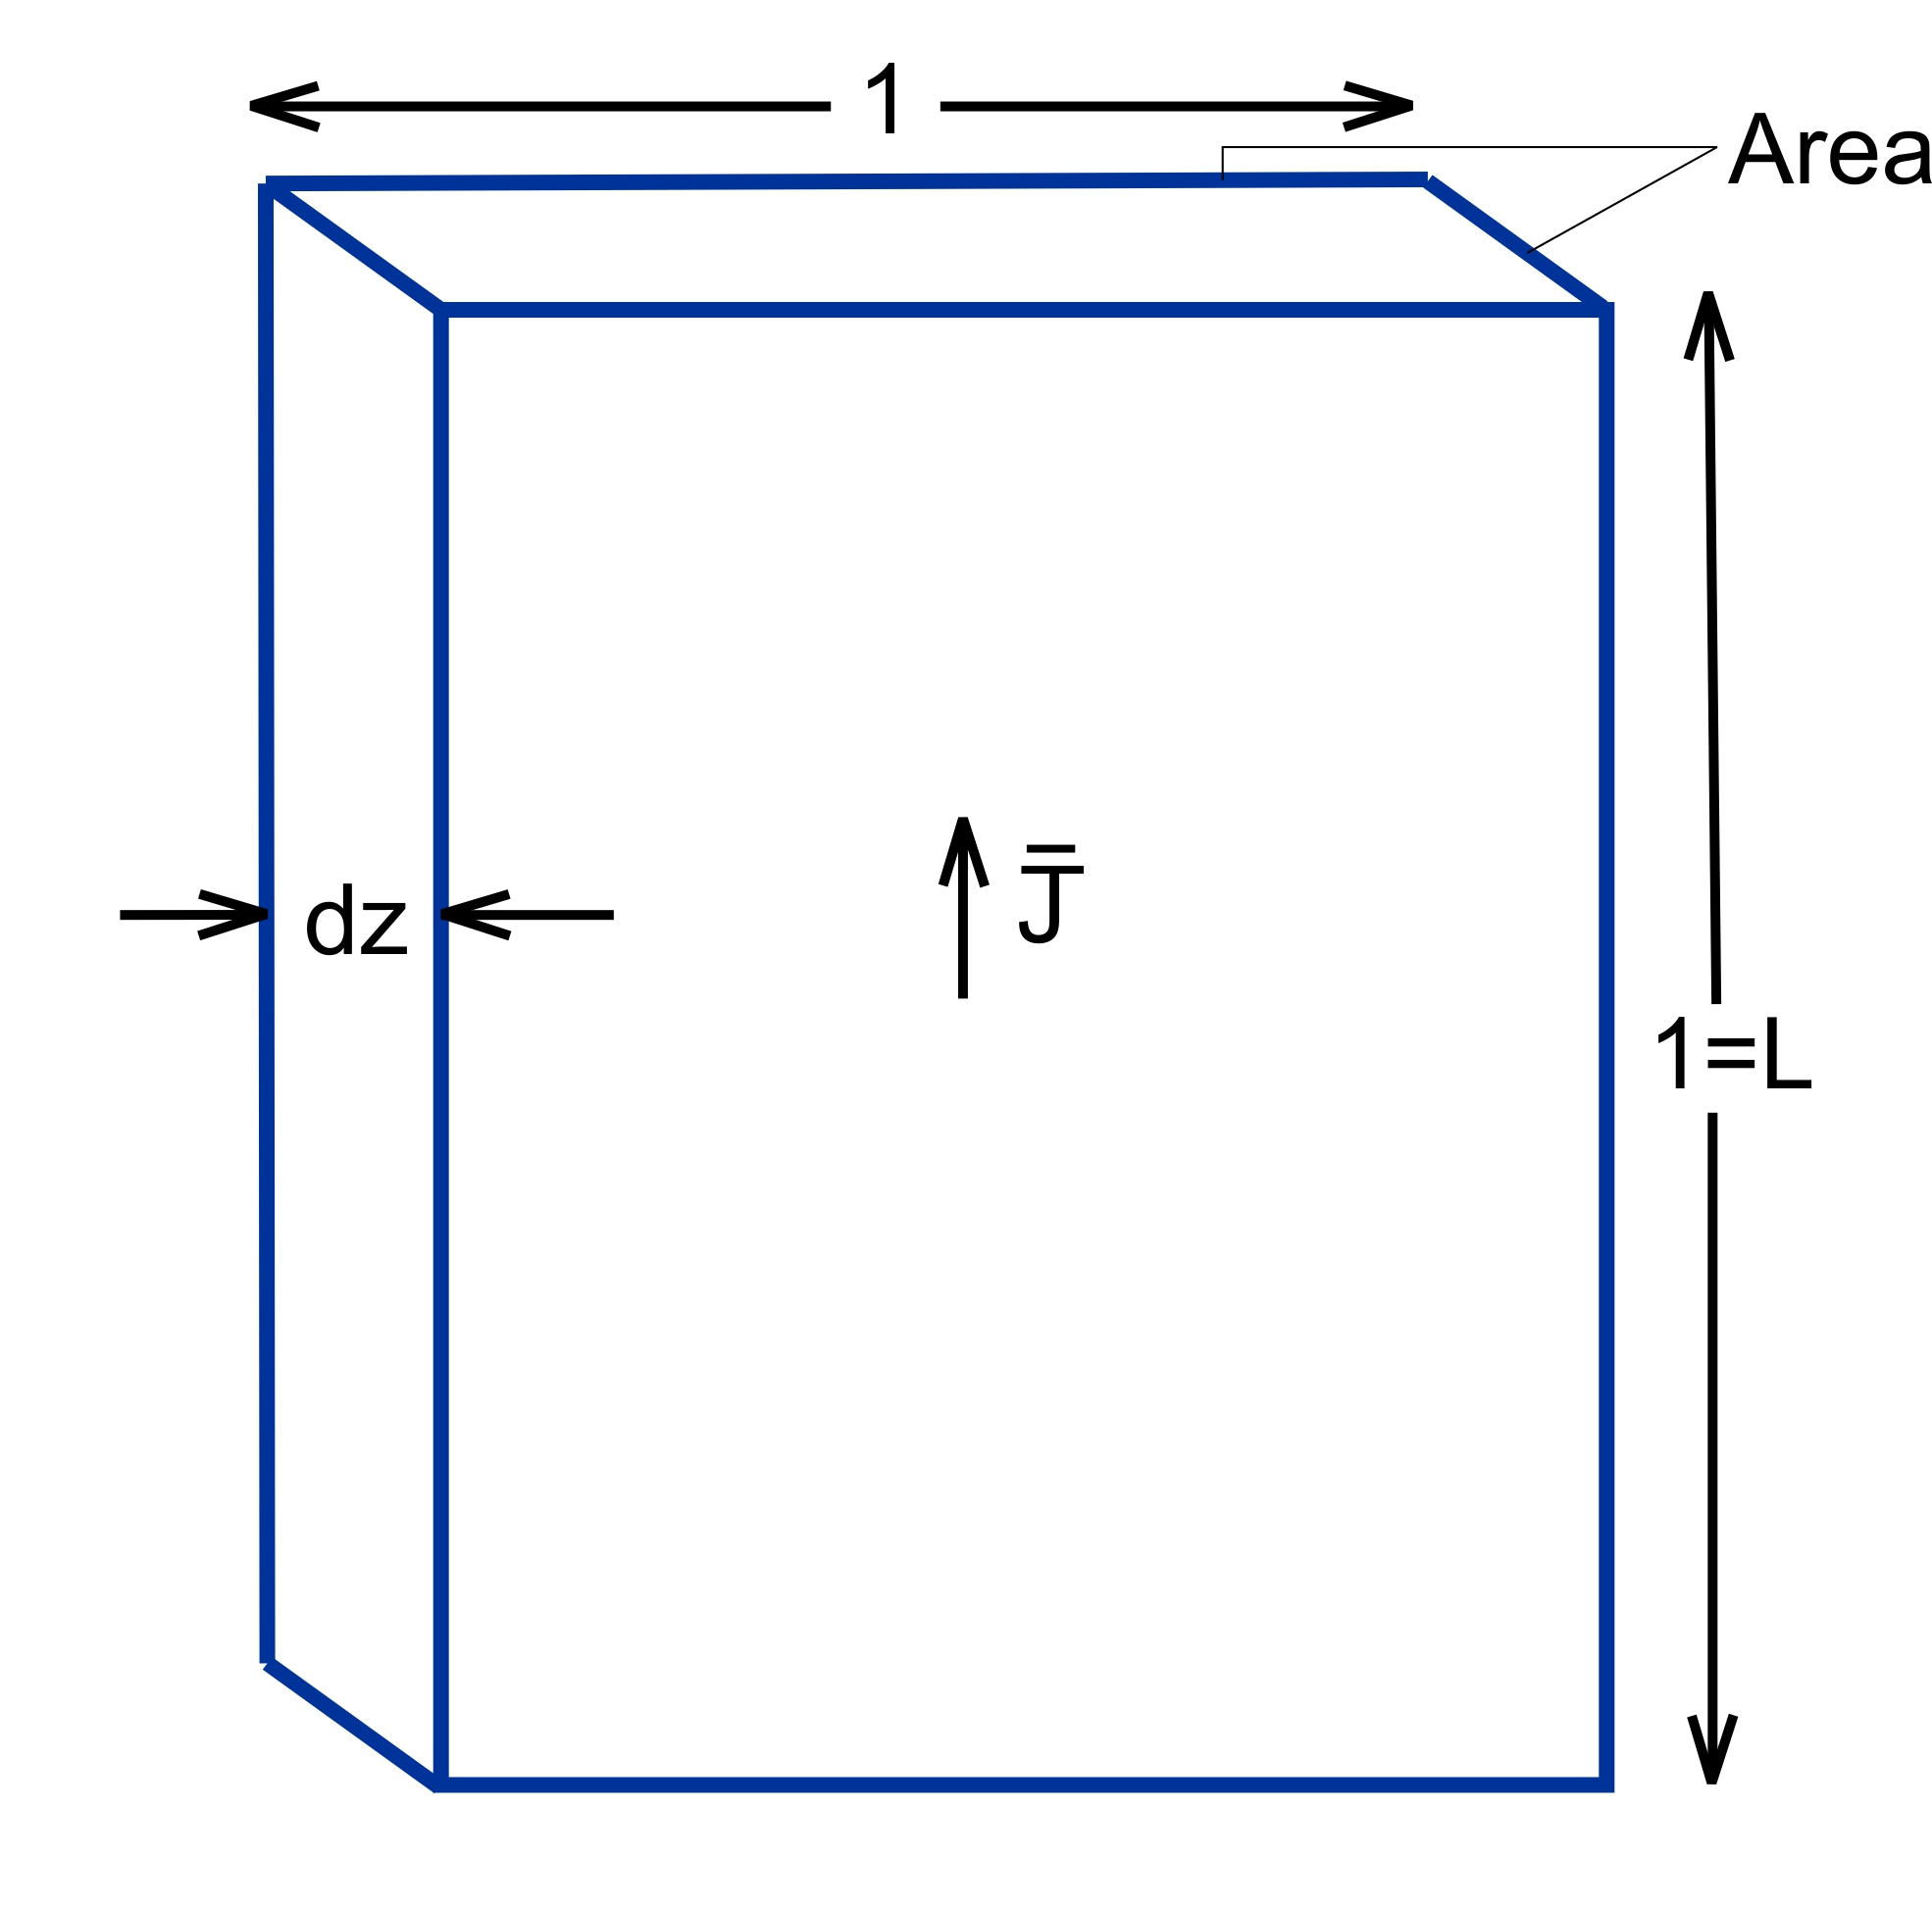
\includegraphics[scale=0.3]{Bello283}}
\caption{A thin slab layer of thickness dz parallel to the surface of the conductor }
\end{figure}
So if we take a thin slab parallel to the surface of the conductor, since we have a finite conduction current we ask how much is the power loss in this thin slab. If we integrate over all depth z, we get the power loss per unit area on the surface of the conductor.\\
Power loss in unit area of conductor.
\begin{align*}
\bar{J}s(1\times\textbf{dz})
\end{align*}
is the current flowing in the direction of  $\bar{J}$s.\\
\begin{center}
The length L is unity 1\\
$\sigma$=conductivity\\
$\dfrac{1}{\sigma}$= resistivity\\
Resistance=$\dfrac{Resistivity \times Length}{Area}$=$\dfrac{1}{\sigma}$$\times$$\dfrac{1}{dz}$=$\dfrac{1}{\sigma dz}$\\\\
current flowing in the area=Jdz\\\\
R=$\dfrac{1}{\sigma dz}$,\ I=Jdz,\ d$\omega$=ohmic loss in slab\\
d$\omega$=$\dfrac{1}{2}$$\lvert$I$\rvert$$^{2}R$\\
I and R can be complex hence $\dfrac{1}{2}$$\lvert$$I\rvert$$^{2}$R\\
\begin{align*}
I=\bar{J}dz
\end{align*}
\begin{align*}
I=\sigma\bar{E}_{0}\textit{e}^{-\gamma z}dz
\end{align*}
\begin{align*}
d\omega=\dfrac{1}{2}\lvert\sigma\bar{E}_{0}\textit{e}^{-\alpha z}\textit{e}^{-j\beta z}\rvert^{2}\times\dfrac{1}{\sigma dz}
\end{align*}
\begin{align*}
d\omega=\dfrac{1}{2}\sigma\lvert\bar{E}_{0}\rvert^{2}\textit{e}^{-2\alpha z}dz
\end{align*}
\end{center}
\begin{Large}
	The total power loss in the whole depth under the unit area of the surface is
\end{Large}
\begin{align}
\omega=\int_{0}^{\infty}\dfrac{1}{2}\sigma\lvert E_{0}\rvert^{2}\textit{e}^{-2\alpha z}dz=\dfrac{1}{2}\sigma\bar{E}_{0}^{2}[\dfrac{\textit{e}^{-2\alpha z}}{-2\alpha}]_{0}^{\infty}
\end{align}
\begin{align}
\omega=\dfrac{1}{2}\dfrac{\sigma}{2\alpha}\lvert E_{0}\rvert^{2}
\end{align}
but
\begin{align}
\gamma=\sqrt{j\omega\mu\sigma}=\alpha+j\beta=\sqrt{\dfrac{\omega\mu\sigma}{2}}+j\sqrt{\dfrac{\omega\mu\sigma}{2}}\\
\dfrac{1}{2}\dfrac{\sigma}{2\sqrt{\dfrac{\omega\mu\sigma}{2}}}\lvert E_{0}\rvert^{2}=\dfrac{1}{2}\dfrac{\sigma}{\sqrt{2\omega\mu\sigma}}\lvert E_{0}\rvert^{2}=\dfrac{1}{2}\dfrac{\sigma}{\sqrt{2}\lvert\gamma\rvert}\lvert E_{0}\rvert^{2}
\end{align}
Again from surface current density,\\
$\bar{J}s=\dfrac{\sigma}{\gamma}E_{0}\hat{x}$\\
$\omega=\dfrac{1}{2}\dfrac{\sigma}{\sqrt{2}\lvert\gamma\rvert}\times \lvert\dfrac{\bar{J}_{s}\gamma}{\sigma}\rvert^{2}$\\\\
recall\ $\lvert$$\gamma$$\rvert$=$\sqrt{\omega\mu\sigma}$
\begin{align}
\omega=\dfrac{1}{2}\times \dfrac{\sigma}{\sqrt{2}\lvert\gamma\rvert}\times \dfrac{\lvert\gamma\rvert^{2}}{\lvert\sigma\rvert^{2}}\times \lvert\bar{J}_{s}\rvert^{2}=\dfrac{1}{2}\times \dfrac{\sigma}{\sqrt{2}\lvert\gamma\rvert}\times \lvert\bar{J}_{s}\rvert^{2}
\end{align}

\begin{align}
\omega=\dfrac{1}{2}\times \dfrac{\sqrt{\omega\mu\sigma}}{\sqrt{2}\sigma}\times \lvert\bar{J}_{s}\rvert^{2}=\dfrac{1}{2}\times \sqrt{\dfrac{\omega\mu}{2\sigma}}\lvert\bar{J}s\rvert^{2}
\end{align}
\begin{align}
Z_{s}=\sqrt{\dfrac{j\omega\mu}{\sigma}}=\sqrt{\dfrac{\omega\mu}{2\sigma}}+j\sqrt{\dfrac{\omega\mu}{2\sigma}}
\end{align}
Hence we say that the surface impedance has a resistive part called the surface resistance and a reactive part called the surface reactance.\\
\begin{align}
Z_{s}=R_{s}+jX_{s}\\	
\omega=\dfrac{1}{2}\times \lvert\bar{J}s\rvert^{2}\times \sqrt{\dfrac{\omega\mu}{2\sigma}}=\dfrac{1}{2}\lvert\bar{J}s\rvert^{2}R_{s}
\end{align}

This is the reason that the power loss per unit area of conducting surface can be obtained if we know the surface current density and the surface resistance.\\

Later on we see that if we go to structures like wave guides, then the conductor loss is calculated from the surface current density, because the conductor surface current density can be obtained from magnetic fields. So if we know the tangential component of magnetic field on the surface of the conductor, we can find out using $\hat{n}$$\times $$\bar{H}$, the linear surface current density with $\bar{J}$s known and Z$_{s}$(surface impedance) known, from there we can find out the power loss per unit area of the conductor.\\

Essentially we have calculated the power loss by using the circuit concept that is, found out the current and the resistance in the slab, then we found out the I$^{2}$R loss, from there we obtained the power loss on the surface of the conductor. We can find same thing by the wave approach. Once we have electric and magnetic field, that is essentially a wave phenomenon going in the z direction. So the power going with the wave into the conductor is essentially the power which is lost into the ohmic loss conductor. This power is finite and is decreasing as the wave travels with time as no power is coming back. So whatever was the power flow inside the conductor is a measure of the power that was lost inside the conductor. So instead of doing the calculation of the power loss from an electrical point of view, by finding out the current and resistance, we can use the wave concept and find out what the power loss is inside the conductor with the interface shown and \textbf{E} and \textbf{H} in direction shown in the image below. Then the power flow as the location shown in the image below. Since we are asking for power flow per unit area of the surface, we find the poynting vector at the surface of the conductor. That is the power which is essentially going into the conductor and which is lost as Ohmic losses in the conductor.\\
Poynting vector,
\begin{align}
\bar{P}=\bar{E}\times \bar{H}=Re\dfrac{1}{2}E_{0}H_{0}^{\ast}\hat{z}
\end{align}
We substitute $\bar{H}$$_{0}$=$\dfrac{E_{0}}{\eta_{c}}$ for this medium
\begin{align}
\bar{P}=\dfrac{\lvert\bar{E}_{0}\rvert^{2}}{2\eta_{c}^{\ast}}\\
\bar{P}=\dfrac{1}{2}\lvert\bar{E}_{0}\rvert^{2}\times \dfrac{1}{\eta_{c}^{\ast}}
\end{align}

Recall  $\eta_{c}=\sqrt{\dfrac{j\omega\mu}{\sigma}}$\\
So that,\\\\
$\eta_{c}&=\sqrt{\dfrac{\omega\mu}{\sigma}}(\dfrac{1}{\sqrt{2}}+j\dfrac{1}{\sqrt{2}})$\\\\
$\eta_{c}^{\ast}&=\sqrt{\dfrac{\omega\mu}{\sigma}}(\dfrac{1}{\sqrt{2}}-j\dfrac{1}{\sqrt{2}})$\\\\

$\eta_{c}=\sqrt{\dfrac{\omega\mu}{\sigma}}(\dfrac{1}{\sqrt{2}}+j\dfrac{1}{\sqrt{2}})$\\\\
$\eta_{c}^{\ast}=\sqrt{\dfrac{\omega\mu}{\sigma}}(\dfrac{1}{\sqrt{2}}-j\dfrac{1}{\sqrt{2}})$\\\\
\begin{align}
\bar{P}=\dfrac{1}{2}\lvert\bar{E}_{0}\rvert^{2}\dot{\dfrac{1}{\sqrt{\dfrac{\omega\mu}{\sigma}}(\dfrac{1}{\sqrt{2}}-j\dfrac{1}{\sqrt{2}})}} 
\end{align}
$=\dfrac{1}{2}\lvert\bar{E}_{0}\rvert^{2}\times \dfrac{\sqrt{\dfrac{\omega\mu}{\sigma}}(\dfrac{1}{\sqrt{2}}+j\dfrac{1}{\sqrt{2}})}{\sqrt{\dfrac{\omega\mu}{\sigma}}(\dfrac{1}{\sqrt{2}}-j\dfrac{1}{\sqrt{2}})\times \sqrt{\dfrac{\omega\mu}{\sigma}}(\dfrac{1}{\sqrt{2}}+j\dfrac{1}{\sqrt{2}})}$\\\\\\
$\bar{P}=\dfrac{1}{2}\lvert\bar{E}_{0}\rvert^{2}Re[\dfrac{\sqrt{\dfrac{\omega\mu}{\sigma}}(\dfrac{1}{\sqrt{2}}+j\dfrac{1}{\sqrt{2}})}{\dfrac{\omega\mu}{\sigma}(\dfrac{1}{2}+\dfrac{1}{2})}]\\\\\\
\bar{P}=\dfrac{1}{2}\lvert\bar{E}_{0}\rvert^{2}Re[\dfrac{\sigma}{\omega\mu}(\sqrt{\dfrac{\omega\mu}{\sigma}}(\dfrac{1}{\sqrt{2}}+j\dfrac{1}{\sqrt{2}}))]$\\\\\\\
$\bar{P}=\dfrac{1}{2}\lvert\bar{E}_{0}\rvert^{2}\times \sqrt{\dfrac{\sigma}{\omega\mu}}\times \dfrac{1}{\sqrt{2}}$\\\\\\
\begin{equation}
\bar{P}=\dfrac{1}{2}\lvert\bar{E}_{0}\rvert^{2}\times \sqrt{\dfrac{\sigma}{2\omega\mu}}
\end{equation}\\

This expression is same as we got for power loss using the surface impedance of the conducting medium. So we can calculate the power loss either by using the circuit concept or the wave concept. Circuit concept by finding $\bar{J}$$_{s}$, find out Ohmic loss or I$^{2}$R loss or use the wave concept to find out what the power going inside the surface of the conductor and that power should essentially get lost inside the conductor. Since the field at z=$\infty$ goes to zero there is no power flow at z=$\infty$, so whatever power went into the conductor must have been lost in the heating of the conductor. So either the electrical circuit concept or the wave concept can be used to find out the power loss per unit area on the surface of the conductor.\\

The power that is being lost inside the conductor is inversely proportional to the conductivity. From P=$\dfrac{1}{2}$$\lvert E_{0}\rvert$$^{2}$$\sqrt{\dfrac{\sigma}{2\omega\mu}}$ we are dealing with waves here. The higher the conductivity of the medium it propagates the more the power loss of this wave, so that in a pure dielectric with $\sigma$=0, it will have no power loss at all in that medium. So, large $\sigma$ means large part of the electromagnetic wave energy is taken by the medium(or lost to the medium). With high frequency, it  losses less of its energy to the medium through which it propagates. So for ideal conductor with $\sigma$$\longrightarrow$$\infty$, the EM wave losses all of its power to this conductor but with skin depth of nearly zero. All of this energy lost flow as pure surface current on this conductor without any Ohmic losses and the entire energy is reflected from the boundary.\footnote{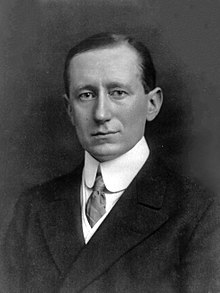
\includegraphics[height=20mm]{footnotegm.jpg}\\Guglielmo Marconi, 1st Marquis of Marconi (25 April 1874 ? 20 July 1937) was an Italian inventor and electrical engineer known for his pioneering work on long-distance radio transmission and for his development of Marconi's law and a radio telegraph system. He is usually credited as the inventor of radio}

For very high frequencies or ideal conductor, $\sigma$=$\infty$, the power will grow identically to zero but for an ideal conductor, there is no power going inside the conductor similarly when the frequency becomes large, there is no power going inside the conductor. What this means is, for high conductivity or high frequency, the resistance penetrating the conductor, the power does not go inside the conductor.\\

In lossy transmission line, the power was getting lost in the heating of the line. In this case the power is dying down rapidly but the power is not lost in the Ohmic loss. The power is not able to penetrate this layer so conductivity=$\infty$. No power penetrates the conductor. It gets reflected.\\

In conclusion, when the conductivity is infinite, the wave just does not penetrate the medium, there is no power loss and the entire energy is reflected to the boundary.
